\chapter{Réacteurs continus et procédés industriels}\label{ch:b2:continuous-reactors}

Au laboratoire, une réaction se conduit dans un ballon~: on introduit les réactifs, on
agite le mélange pendant une heure, on arrête la réaction et on isole le produit.
Une usine qui fabrique le même produit par milliers de tonnes travaille
autrement. Son réacteur ne se vide jamais~: les réactifs entrent d'un côté, les
produits sortent de l'autre, jour et nuit, et la composition à l'intérieur
ne change pas au cours du temps. Deux questions remplacent alors «~combien de temps~?~»~:
quelle taille doit avoir le réacteur pour une \omterm{def:b2:continuous-reactors:conversion}{conversion} donnée, et comment évacuer la chaleur
de la réaction avant qu'elle ne fasse s'emballer le réacteur~? Ce
chapitre écrit les bilans de matière et d'énergie des deux \omterm{def:b2:continuous-reactors:reactors}{réacteurs continus}
idéaux, la cuve agitée et le tube, les compare, et
montre qu'un réacteur peut avoir plusieurs états possibles, dont l'un est un
emballement.

\begin{recall}
Le volume de première année~: vitesse de réaction, lois de vitesse et ordres, lois intégrées
d'un réacteur fermé (appelé désormais \omterm{def:b2:continuous-reactors:reactors}{réacteur discontinu}), temps de demi-réaction, la loi
d'Arrhenius $k = A\,\mathrm e^{-E_a/RT}$, réactions successives.
\Cref{ch:b2:reaction-enthalpy}~: chaleur libérée à pression constante~;
\cref{ch:b2:equilibrium-shifts}~: \omterm{def:b2:equilibrium-shifts:single-pass}{conversion par passage}, \omterm{def:b2:equilibrium-shifts:single-pass}{recyclage}. En
physique~: le bilan d'un système ouvert en écoulement permanent (ce qui entre moins
ce qui sort est égal à ce qui s'accumule).
\end{recall}

\begin{omfigure}
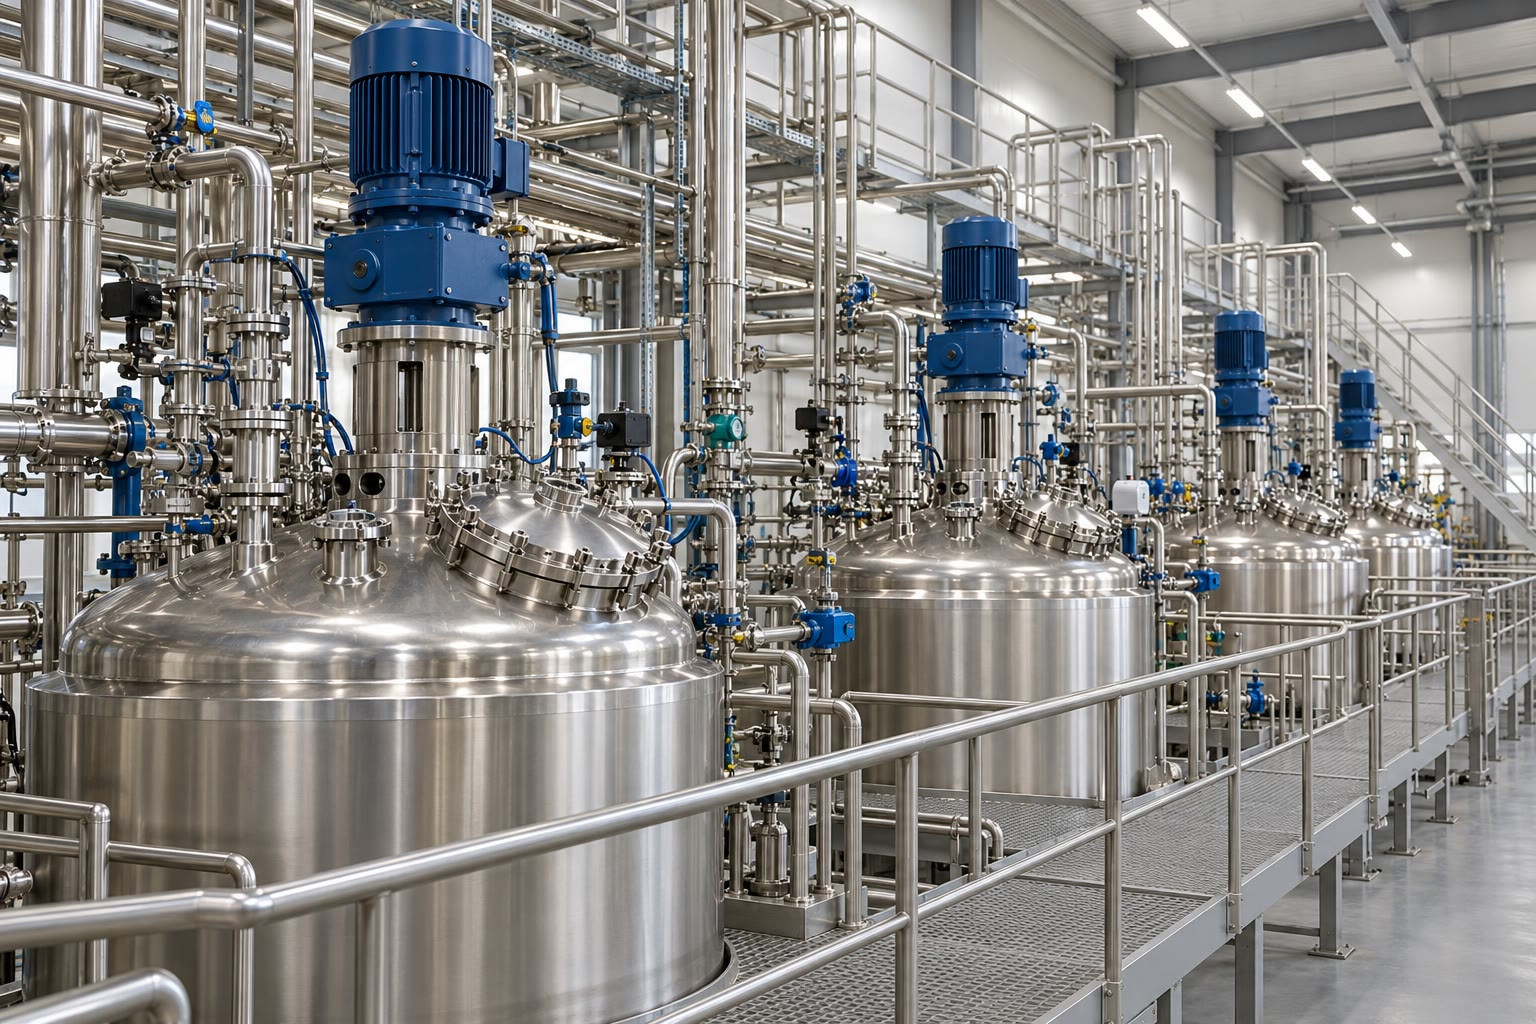
\includegraphics[width=0.6\linewidth]{images/book3/ai/b2-05-stirred-tanks.jpg}

{\small Réacteurs à cuve agitée dans une usine chimique~: chaque cuve porte son
moteur et son réducteur, l'arbre de l'agitateur plongeant dans le mélange réactionnel~;
les canalisations amènent les alimentations et emportent le produit et l'eau de refroidissement.}
\end{omfigure}

\section{Du réacteur discontinu au réacteur continu}

\begin{definition}[Types de réacteurs]\label{def:b2:continuous-reactors:reactors}
Un \emph{réacteur discontinu}\index{reacteur discontinu@réacteur discontinu} est une enceinte fermée dans laquelle la
réaction se déroule sans entrée ni sortie de matière. Un
\emph{réacteur continu}\index{reacteur continu@réacteur continu} est traversé par un écoulement
permanent de matière. Deux réacteurs continus idéaux servent de modèles~:
\begin{itemize}
  \item le \emph{réacteur parfaitement agité continu}\index{reacteur parfaitement agite continu@réacteur parfaitement agité continu}
(RPAC), si bien agité que son contenu est
        uniforme, et donc identique au flux qui en sort~;
  \item le \emph{réacteur en écoulement piston}\index{reacteur en ecoulement piston@réacteur en écoulement piston} (RP), un tube
        traversé par le fluide sans mélange dans le sens de l'écoulement, chaque tranche de
        fluide avançant comme un piston pendant qu'elle réagit.
\end{itemize}
\end{definition}

On dit qu'un \omterm{def:b2:continuous-reactors:reactors}{réacteur continu} fonctionne en \emph{régime permanent} lorsque
rien en son sein ne varie au cours du temps~: les débits, les températures et les
compositions en chaque point sont constants. On considère une seule réaction
$\mathrm A \to$ produits, une alimentation liquide de masse volumique constante (le
débit volumique $Q_v$ est donc le même à l'entrée et à la sortie), de
concentration $c_{A,0}$ à l'entrée.

\begin{definition}[Temps de passage]\label{def:b2:continuous-reactors:residence-time}
Le \emph{temps de passage}\index{temps de passage} d'un \omterm{def:b2:continuous-reactors:reactors}{réacteur continu} de
volume $V$ alimenté au débit volumique $Q_v$ est $\tau = V/Q_v$~: le temps
moyen qu'un volume de fluide passe à l'intérieur.
\end{definition}

\begin{definition}[Taux de conversion]\label{def:b2:continuous-reactors:conversion}
Le \emph{taux de conversion}\index{taux de conversion} du réactif A est $X = (F_{A,0} -
F_A)/F_{A,0}$, où $F_{A,0}$ et $F_A$ sont les débits molaires de A
à l'entrée et à la sortie du réacteur~; pour un \omterm{def:b2:continuous-reactors:reactors}{réacteur discontinu}, $X = (n_{A,0} -
n_A)/n_{A,0}$. À masse volumique constante, $X = 1 - c_A/c_{A,0}$.
\end{definition}

Le \omterm{def:b2:continuous-reactors:conversion}{taux de conversion} se rapporte à un réactif, et à un réacteur ou à un passage~; le
taux d'avancement final du volume de première année se rapporte à une réaction et à son
réactif limitant. Pour une réaction unique dont le réactif limitant est A, les
deux coïncident.

\begin{proposition}[Réacteur discontinu]\label{prop:b2:continuous-reactors:batch}
Dans un \omterm{def:b2:continuous-reactors:reactors}{réacteur discontinu} de volume constant, une réaction d'ordre 1 atteint le
\omterm{def:b2:continuous-reactors:conversion}{taux de conversion} $X = 1 - \mathrm e^{-kt}$ au bout de la durée $t$, et une réaction d'ordre 2
de concentrations initiales égales $c_0$ le taux $X =
kc_0t/(1 + kc_0t)$.
\end{proposition}

\begin{proof}
Ce sont les lois de vitesse intégrées du volume de première année, $c_A = c_{A,0}
\mathrm e^{-kt}$ et $1/c_A = 1/c_{A,0} + kt$, écrites avec $X = 1 -
c_A/c_{A,0}$.
\end{proof}

\section{Le réacteur parfaitement agité continu}

\begin{omfigure}
\begin{tikzpicture}[font=\small, >={Stealth}]
  % batch
  \pic[transform shape] at (0,0) {rbflask={0.6}{omDef!20}};
  \node[below] at (0,-0.15) {discontinu};
  % CSTR
  \begin{scope}[xshift=4.2cm]
    \draw[thick, fill=omDef!15] (-1.2,0) rectangle (1.2,2.4);
    \draw[thick] (0,3.0) -- (0,0.5);
    \draw[thick, fill=gray!40] (-0.5,0.45) rectangle (0.5,0.6);
    \draw[thick, fill=gray!30] (-0.25,3.0) rectangle (0.25,3.35);
    \draw[->, thick, omDef] (-2.8,2.0) -- (-1.2,2.0) node[pos=0.0, above, anchor=south west, inner sep=1pt] {$Q_v$, $c_{A,0}$};
    \draw[->, thick, omThm] (1.2,0.3) -- (2.5,0.3) node[pos=1, below] {$Q_v$, $c_A$};
    \node[fill=omDef!15, inner sep=1pt] at (0.62,1.5) {$V$, $c_A$};
    \node[below] at (0,-0.15) {cuve agitée};
  \end{scope}
  % PFR
  \begin{scope}[xshift=8.4cm, yshift=1.0cm]
    \draw[thick, fill=omDef!10] (0,0) rectangle (4.2,0.7);
    \fill[omThm!25] (2.0,0) rectangle (2.35,0.7);
    \draw[thick] (2.0,0) -- (2.0,0.7) (2.35,0) -- (2.35,0.7);
    \node[above] at (2.17,0.75) {$\dd V$};
    \draw[->, thick, omDef] (-0.9,0.35) -- (0,0.35) node[pos=0, above] {$F_{A,0}$};
    \draw[->, thick, omThm] (4.2,0.35) -- (5.0,0.35) node[pos=1, above] {$F_A$};
    \node[below] at (1.0,0) {$F_A(V)$};
    \node[below] at (2.1,-1.15) {tube à écoulement piston};
  \end{scope}
\end{tikzpicture}

{\small Les trois réacteurs idéaux. Un ballon en régime discontinu~; une cuve agitée dont le contenu
uniforme est celui du flux de sortie~; un tube parcouru en écoulement piston, dans
lequel le débit de A diminue d'une tranche à l'autre.}
\end{omfigure}

\begin{proposition}[Bilan d'une cuve agitée]\label{prop:b2:continuous-reactors:cstr-balance}
En régime permanent, une cuve agitée de volume $V$ dans laquelle A disparaît à
la vitesse $r$ (en mol par litre et par seconde) vérifie
\[
  F_{A,0} - F_A - rV = 0, \qquad\text{c'est-à-dire}\qquad c_{A,0} - c_A = r\,\tau ,
\]
la vitesse étant évaluée à la composition et à la température de sortie.
\end{proposition}

\begin{proof}
Bilan de A sur la cuve pendant $\dd t$~: ce qui entre, $F_{A,0}\dd t$,
moins ce qui sort, $F_A\dd t$, moins ce qui réagit, $rV\dd t$, est égal à
l'accumulation, nulle en régime permanent. La cuve étant uniforme, la vitesse est
la même partout et égale à celle du flux de sortie. Il reste à diviser par $Q_v$.
\end{proof}

\begin{theorem}[Conversion dans une cuve agitée]\label{thm:b2:continuous-reactors:cstr}
Pour une réaction d'ordre 1, $X = \dfrac{k\tau}{1 + k\tau}$~; pour une
réaction d'ordre 2 dont les deux réactifs sont introduits à la même concentration $c_0$,
$X$ est la racine dans $[0, 1]$ de $Da\,(1 - X)^2 = X$, avec $Da =
kc_0\tau$.
\end{theorem}

\begin{proof}
Ordre 1~: $r = kc_A$, donc $c_{A,0} - c_A = k\tau c_A$, $c_A = c_{A,0}/(1 + k\tau)$
et $X = 1 - 1/(1 + k\tau)$. Ordre 2~: $r = kc_A^2$ (les deux concentrations restent
égales), $c_0X = k\tau c_0^2(1 - X)^2$.
\end{proof}

Le groupement sans dimension $Da = k\tau$ (ou $kc_0\tau$), le nombre de
Damköhler, compare le \omterm{def:b2:continuous-reactors:residence-time}{temps de passage} au temps caractéristique de la réaction~:
il fixe à lui seul le \omterm{def:b2:continuous-reactors:conversion}{taux de conversion}.

\begin{method}[Dimensionner un réacteur]\label{met:b2:continuous-reactors:size-reactor}
\begin{enumerate}
  \item Écrire la loi de vitesse et le \omterm{def:b2:continuous-reactors:conversion}{taux de conversion} $X$ visé.
  \item À partir du bilan du réacteur choisi, déterminer le nombre de Damköhler
        qui donne $X$.
  \item En déduire $\tau$ à partir de $Da$ et de la constante de vitesse à la température
        de travail, puis $V = \tau Q_v$ à partir du débit à traiter.
\end{enumerate}
\end{method}

\section{Le réacteur en écoulement piston}

\begin{theorem}[Conversion dans un réacteur en écoulement piston]\label{thm:b2:continuous-reactors:pfr}
En régime permanent, le débit de A le long d'un tube à écoulement piston vérifie
$\dd F_A/\dd V = -r$. Pour une réaction d'ordre 1, cela donne $X = 1 -
\mathrm e^{-k\tau}$, et pour une réaction d'ordre 2 à alimentations égales $X =
Da/(1 + Da)$~: ce sont les lois du \omterm{def:b2:continuous-reactors:reactors}{réacteur discontinu}, avec le \omterm{def:b2:continuous-reactors:residence-time}{temps de passage} à la
place du temps.
\end{theorem}

\begin{proof}
Bilan de A sur la tranche comprise entre $V$ et $V + \dd V$~: $F_A(V) - F_A(V + \dd V)
- r\,\dd V = 0$, d'où l'équation différentielle. Avec $F_A = Q_vc_A$ et
$\dd V = Q_v\,\dd t'$ (la durée $t'$ qu'une tranche a passée dans le tube), elle s'écrit
$\dd c_A/\dd t' = -r$~: chaque tranche est un petit \omterm{def:b2:continuous-reactors:reactors}{réacteur discontinu} qui reste dans le
tube pendant $\tau$. La séparation des variables pour $r = kc_A$ donne $c_A = c_{A,0}
\mathrm e^{-k\tau}$ à la sortie~; pour $r = kc_A^2$, $1/c_A - 1/c_0 = k\tau$.
\end{proof}

\begin{omfigure}
\begin{tikzpicture}
\begin{axis}[
  width=0.75\linewidth, height=6cm, xmin=0, xmax=10, ymin=0, ymax=1.05,
  axis x line=bottom, axis y line=left, xlabel={nombre de Damköhler $k\tau$},
  ylabel={taux de conversion $X$}, tick label style={font=\small},
  label style={font=\small}, clip=false,
  legend style={font=\scriptsize, draw=none, at={(0.98,0.05)}, anchor=south east}]
\addplot[omThm, very thick] table[x=Da, y=pfr] {figdata/out/bachelor-2-reactors-a.dat};
\addplot[omProp, thick] table[x=Da, y=five] {figdata/out/bachelor-2-reactors-a.dat};
\addplot[omProp, thick, dashed] table[x=Da, y=two] {figdata/out/bachelor-2-reactors-a.dat};
\addplot[omDef, very thick] table[x=Da, y=cstr] {figdata/out/bachelor-2-reactors-a.dat};
\legend{écoulement piston, 5 cuves en série, 2 cuves en série, 1 cuve agitée}
\draw[dotted] (axis cs:2.303,0) -- (axis cs:2.303,0.9) -- (axis cs:9,0.9);
\fill[omThm] (axis cs:2.303,0.9) circle (1.4pt);
\fill[omDef] (axis cs:9,0.9) circle (1.4pt);
\end{axis}
\end{tikzpicture}

{\small \omterm{def:b2:continuous-reactors:conversion}{Taux de conversion} d'une réaction d'ordre 1 en fonction de $k\tau$ dans les réacteurs
idéaux. Pour 90\,\% de \omterm{def:b2:continuous-reactors:conversion}{conversion}, un tube à écoulement piston exige $k\tau = \ln 10 = 2.3$,
une seule cuve agitée $k\tau = 9$~: quatre fois le volume. Des cuves en série
se rapprochent du tube.}
% (model curves, computed in figdata/bachelor-2/reactors.py)
\end{omfigure}

\begin{proposition}[Cuve ou tube]\label{prop:b2:continuous-reactors:compare}
Pour toute vitesse qui croît avec la concentration de A (tout ordre
positif), un \omterm{def:b2:continuous-reactors:reactors}{réacteur en écoulement piston} atteint un \omterm{def:b2:continuous-reactors:conversion}{taux de conversion} donné avec un volume plus petit
qu'une cuve agitée.
\end{proposition}

\begin{proof}
D'après les bilans, $\tau_{\text{RPAC}} = c_{A,0}X/r(X)$ (la vitesse à la composition
de sortie) et $\tau_{\text{RP}} = c_{A,0}\int_0^X\dd X'/r(X')$. Comme $r$
décroît quand $X$ croît, $1/r(X') \leq 1/r(X)$ sur $[0, X]$~: l'intégrale
vaut au plus $X/r(X)$. Graphiquement, sur un diagramme de $1/r$ en fonction de $X$, le
$\tau$ du tube est l'aire sous la courbe et celui de la cuve le rectangle de
hauteur $1/r(X)$ (figure ci-dessous). Pour l'ordre 1~: $\ln(1 + k\tau) \leq k\tau$, le
même énoncé sous une autre forme.
\end{proof}

La cuve agitée travaille entièrement à la concentration de sortie, la plus basse
du système, et donc à la vitesse la plus faible~; le tube profite des fortes concentrations
près de son entrée. Les avantages de la cuve sont ailleurs~: une température uniforme et
facile à régler, et un fonctionnement simple.

\begin{omfigure}
\begin{tikzpicture}
\begin{axis}[
  width=0.62\linewidth, height=5.6cm, xmin=0, xmax=1, ymin=0, ymax=22,
  axis x line=bottom, axis y line=left, xlabel={taux de conversion $X$},
  ylabel={$1/r$ (unités du modèle)}, tick label style={font=\small},
  label style={font=\small}, clip=false]
\fill[omDef!15] (axis cs:0,0) rectangle (axis cs:0.9,10);
\addplot[omThm, fill=omThm!20, draw=none, domain=0:0.9, samples=60] {1/(1-x)} \closedcycle;
\addplot[black, very thick] table[x=X, y=invr] {figdata/out/bachelor-2-reactors-c.dat};
\draw[omDef, thick] (axis cs:0,10) -- (axis cs:0.9,10) -- (axis cs:0.9,0);
\node[omDef, font=\scriptsize, anchor=south] at (axis cs:0.45,10.2) {cuve agitée~: rectangle, $\tau = 9$};
\node[omThm, font=\scriptsize, anchor=west] (pf) at (axis cs:0.05,6.5) {écoulement piston~: aire grisée, $\tau = \ln 10$};
\draw[omThm, ->] (axis cs:0.25,6.0) -- (axis cs:0.3,0.8);
\end{axis}
\end{tikzpicture}

{\small Diagramme de Levenspiel d'une réaction d'ordre 1 ($k = 1$, $c_{A,0} = 1$).
Pour 90\,\% de \omterm{def:b2:continuous-reactors:conversion}{conversion}, la cuve agitée a besoin du rectangle entier, l'écoulement
piston seulement de l'aire grisée sous la courbe.}
% (model, computed in figdata/bachelor-2/reactors.py)
\end{omfigure}

\begin{proposition}[Cuves en série]\label{prop:b2:continuous-reactors:cascade}
$N$ cuves agitées identiques en série, de \omterm{def:b2:continuous-reactors:residence-time}{temps de passage} total $\tau$, convertissent une
réaction d'ordre 1 avec le taux $X_N = 1 - (1 + k\tau/N)^{-N}$, qui croît avec
$N$ et tend vers la valeur de l'écoulement piston, $1 - \mathrm e^{-k\tau}$.
\end{proposition}

\begin{proof}
Chaque cuve divise la concentration par $1 + k\tau/N$. Et $(1 +
k\tau/N)^{-N} = \exp[-N\ln(1 + k\tau/N)] \to \mathrm e^{-k\tau}$, puisque
$N\ln(1 + u/N) \to u$.
\end{proof}

\begin{definition}[Sélectivité]\label{def:b2:continuous-reactors:selectivity}
Lorsqu'un réactif peut donner plusieurs produits, la \emph{sélectivité}\index{selectivite@sélectivité}
en produit désiré B est la quantité de B formée divisée par la quantité de
réactif consommée (multipliée par le rapport stœchiométrique)~: elle indique quelle part de
ce qui a réagi a pris la bonne voie.
\end{definition}

\begin{proposition}[Un intermédiaire dans une cuve et dans un tube]\label{prop:b2:continuous-reactors:consecutive}
Pour des réactions successives d'ordre 1 $\mathrm A \xrightarrow{k_1} \mathrm B
\xrightarrow{k_2} \mathrm C$, avec une alimentation en A seul, la concentration
de B en sortie est maximale pour $\tau = \ln(k_2/k_1)/(k_2 - k_1)$ dans un
\omterm{def:b2:continuous-reactors:reactors}{réacteur en écoulement piston} et pour $\tau = 1/\sqrt{k_1k_2}$ dans une cuve agitée~; le
maximum est plus élevé dans le tube.
\end{proposition}

\begin{proof}
Tube~: on applique les lois du \omterm{def:b2:continuous-reactors:reactors}{réacteur discontinu} vues dans le volume de première année, $c_B = c_{A,0}\frac{k_1}{k_2 - k_1}
(\mathrm e^{-k_1\tau} - \mathrm e^{-k_2\tau})$, maximale là où la dérivée
s'annule, $k_1\mathrm e^{-k_1\tau} = k_2\mathrm e^{-k_2\tau}$. Cuve~: $c_A =
c_{A,0}/(1 + k_1\tau)$ et le bilan de B, $c_B = k_1\tau c_A - k_2\tau c_B$,
donne $c_B = c_{A,0}k_1\tau/[(1 + k_1\tau)(1 + k_2\tau)]$, dont la dérivée
s'annule lorsque $k_1k_2\tau^2 = 1$. La comparaison des maximums fait l'objet de
l'\cref{exo:b2:continuous-reactors:10}.
\end{proof}

\section{Bilan thermique et sécurité}

\begin{definition}[Élévation adiabatique de température]\label{def:b2:continuous-reactors:adiabatic-rise}
L'\emph{élévation adiabatique de température}\index{elevation adiabatique de temperature@élévation adiabatique de température}
$\Delta T_{\text{ad}}$ d'un mélange réactionnel est l'élévation de température qu'il
subirait si la réaction était totale et qu'aucune chaleur n'était évacuée.
\end{definition}

\begin{proposition}[Élévation adiabatique d'un mélange liquide]\label{prop:b2:continuous-reactors:adiabatic}
Pour un mélange de masse volumique $\rho$ et de capacité thermique massique $c_p$, dans lequel
le réactif A, à la concentration $c_{A,0}$, réagit avec l'enthalpie
$\Delta_r H$ par mole de A, l'élévation de température au \omterm{def:b2:continuous-reactors:conversion}{taux de conversion} $X$ sans
perte de chaleur vaut
\[
  \Delta T = \frac{(-\Delta_r H)\,c_{A,0}\,X}{\rho\,c_p}, \qquad
  \Delta T_{\text{ad}} = \frac{(-\Delta_r H)\,c_{A,0}}{\rho\,c_p} .
\]
\end{proposition}

\begin{proof}
Pour une unité de volume, la chaleur libérée, $(-\Delta_r H)c_{A,0}X$, chauffe une
masse $\rho$ de capacité thermique $c_p$ (premier principe à pression constante, les deux
étapes de la \cref{prop:b2:reaction-enthalpy:flame}).
\end{proof}

Un mélange dilué est sans danger~: quelques degrés d'élévation. Un mélange concentré et fortement
\omterm{def:b2:reaction-enthalpy:exothermic}{exothermique} peut s'échauffer de centaines de kelvins, assez pour faire bouillir le
solvant ou déclencher une autre réaction. Et la vitesse croît exponentiellement avec la
température~: la chaleur accélère la réaction, qui libère la chaleur plus vite.

\begin{proposition}[États stationnaires d'une cuve agitée refroidie]\label{prop:b2:continuous-reactors:steady-states}
Pour une cuve agitée alimentée à $T_0$, refroidie par une double enveloppe à $T_0$ de
produit coefficient de transfert thermique par surface $UA$, les températures stationnaires possibles
$T$ sont les solutions de
\[
  \underbrace{\Delta T_{\text{ad}}\,X(T)}_{\text{chaleur produite}} =
  \underbrace{(1 + \kappa)(T - T_0)}_{\text{chaleur évacuée}}, \qquad
  \kappa = \frac{UA}{Q_v\rho c_p},
\]
où $X(T) = k(T)\tau/(1 + k(T)\tau)$ pour une réaction d'ordre 1. La production est
une courbe en S de $T$, l'évacuation une droite~: il peut y avoir une ou trois
intersections.
\end{proposition}

\begin{proof}
Bilan d'énergie de la cuve en régime permanent, par unité de temps~: la chaleur
libérée par la réaction, $(-\Delta_r H)F_{A,0}X$, part avec le flux de
sortie, chauffé de $T_0$ à $T$, $Q_v\rho c_p(T - T_0)$, et à travers
la double enveloppe, $UA(T - T_0)$. Il reste à diviser par $Q_v\rho c_p$. Avec la loi d'Arrhenius,
$X(T)$ passe de 0 à 1 sur un intervalle étroit de température~: un S.
\end{proof}

\begin{omfigure}
\begin{tikzpicture}
\begin{axis}[
  width=0.75\linewidth, height=6.2cm, xmin=300, xmax=470, ymin=0, ymax=250,
  axis x line=bottom, axis y line=left, xlabel={température de la cuve $T$ (K)},
  ylabel={chaleur par unité de débit (K)}, tick label style={font=\small},
  label style={font=\small}, clip=true]
\addplot[omThm, very thick] table[x=T, y=gen] {figdata/out/bachelor-2-reactors-b.dat};
\addplot[omDef, very thick] table[x=T, y=rem] {figdata/out/bachelor-2-reactors-b.dat};
\fill[black] (axis cs:300.03,0.04) circle (2pt);
\fill[white, draw=black] (axis cs:390.4,135.6) circle (2pt);
\fill[black] (axis cs:429.6,194.4) circle (2pt);
\node[font=\scriptsize, anchor=north west, fill=white, inner sep=1pt] at (axis cs:318,58) {froid, stable}; \draw[black!60] (axis cs:301.5,2) -- (axis cs:318,52);
\node[font=\scriptsize, anchor=north west] at (axis cs:393,132) {instable};
\node[font=\scriptsize, anchor=south east] at (axis cs:426,197) {chaud, stable};
\node[omThm, font=\scriptsize, anchor=north west] at (axis cs:440,196) {produite};
\node[omDef, font=\scriptsize, anchor=south east] at (axis cs:452,232) {évacuée};
\end{axis}
\end{tikzpicture}

{\small Diagramme de Semenov d'une cuve agitée refroidie (paramètres d'un modèle). La
chaleur produite (en rouge) et la chaleur évacuée (droite bleue) se coupent trois fois. L'état
du milieu est instable~: un peu plus chaude, la production l'emporte et la cuve
s'emballe vers l'état chaud~; un peu plus froide, elle retombe vers l'état
froid.}
% (model, computed in figdata/bachelor-2/reactors.py)
\end{omfigure}

La stabilité de chaque état découle des pentes~: en une intersection
où la droite d'évacuation est plus raide que la courbe de production, une petite élévation de
température évacue plus de chaleur qu'elle n'en produit, et la cuve se refroidit~;
là où la courbe de production est plus raide, une petite élévation s'entretient d'elle-même. (L'analyse
rigoureuse linéarise les bilans dépendant du temps~; elle est admise
ici.)

\begin{definition}[Emballement thermique]\label{def:b2:continuous-reactors:runaway}
Un \emph{emballement thermique}\index{emballement thermique} est l'élévation auto-accélérée
de la température d'un mélange réactionnel dont la production de chaleur, croissant
exponentiellement avec la température, dépasse l'évacuation de chaleur.
\end{definition}

\begin{method}[Bilan thermique d'un réacteur]\label{met:b2:continuous-reactors:heat-balance}
\begin{enumerate}
  \item Calculer l'\omterm{def:b2:continuous-reactors:adiabatic-rise}{élévation adiabatique de température}~: si elle est de quelques kelvins, le
        réacteur est thermiquement sûr.
  \item Sinon, calculer la puissance de refroidissement, $(-\Delta_r H)F_{A,0}X$ moins la
        chaleur emportée par le flux de sortie, et vérifier que la double enveloppe ou le serpentin
        peut l'évacuer.
  \item Vérifier la stabilité du point de fonctionnement (pentes sur un diagramme de
        Semenov), et ce qui se passerait en cas de panne du refroidissement~: la
        température maximale atteinte, $T + \Delta T_{\text{ad}}(1 - X)$ pour
        le réactif encore présent.
\end{enumerate}
\end{method}

\section{Du protocole à l'usine}

Une synthèse qui fonctionne dans un ballon de \qty{1}{L} ne se transpose pas simplement
à une échelle mille fois plus grande. Le volume, et la chaleur libérée, croissent comme le cube de la
taille~; la paroi, par laquelle la chaleur s'échappe, comme son carré. Une cuve dix
fois plus large a mille fois plus de volume mais seulement cent fois plus de
surface de refroidissement~: une réaction restée tiède dans le ballon peut s'emballer dans
la cuve. La pratique industrielle consiste donc à ajouter lentement le réactif le plus réactif
(la réaction ne peut pas libérer plus de chaleur que le réactif introduit), à diluer,
à refroidir par des serpentins internes, ou à passer à des \omterm{def:b2:continuous-reactors:reactors}{réacteurs continus} de petit volume,
dont la faible rétention limite ce qui peut mal tourner.

La \omterm{def:b2:continuous-reactors:selectivity}{sélectivité} est l'autre préoccupation. Une usine ne jette pas ce qui n'a pas
réagi~: elle sépare le produit et recycle les réactifs, comme dans la
boucle de l'ammoniac. Elle peut donc accepter une \omterm{def:b2:equilibrium-shifts:single-pass}{conversion par passage} modeste si la
\omterm{def:b2:continuous-reactors:selectivity}{sélectivité} est élevée, puisque chaque sous-produit est une matière première perdue et un déchet à
traiter.

\begin{inthelab}[Une cuve agitée sur la paillasse]
La cinétique d'une réaction destinée à une installation continue se mesure dans un
petit réacteur agité alimenté par deux pompes étalonnées, avec une cellule conductimétrique
ou un spectromètre en ligne à la sortie. Faire varier le débit fait varier $\tau$~;
la concentration de sortie stationnaire à chaque $\tau$ donne directement la vitesse, par le
bilan $r = (c_{A,0} - c_A)/\tau$, sans aucune intégration.
\end{inthelab}

\section{Exercices}

\begin{exercise}[$\star$]\label{exo:b2:continuous-reactors:1}
Une cuve agitée de \qty{2.0}{m^3} est alimentée à \qty{0.50}{L/s}. Calculer son
\omterm{def:b2:continuous-reactors:residence-time}{temps de passage} en secondes et en heures.
\end{exercise}

\begin{exercise}[$\star$]\label{exo:b2:continuous-reactors:2}
Une réaction d'ordre 1 a pour constante $k = \qty{1.2e-3}{s^{-1}}$ à la température
de travail. Calculer le \omterm{def:b2:continuous-reactors:conversion}{taux de conversion} dans une cuve agitée et dans un tube à écoulement piston
de même \omterm{def:b2:continuous-reactors:residence-time}{temps de passage}, \qty{30}{min}.
\end{exercise}

\begin{exercise}[$\star$]\label{exo:b2:continuous-reactors:3}
Quel \omterm{def:b2:continuous-reactors:residence-time}{temps de passage} en écoulement piston donne 99\,\% de \omterm{def:b2:continuous-reactors:conversion}{conversion} d'une réaction
d'ordre 1 de constante $k = \qty{0.020}{s^{-1}}$~? Et dans une cuve agitée~?
\end{exercise}

\begin{exercise}[$\star$]\label{exo:b2:continuous-reactors:4}
Une solution aqueuse à \qty{0.50}{mol/L} d'un réactif dont la réaction
libère \qty{-120}{kJ/mol} ($\rho = \qty{1.0}{kg/L}$, $c_p =
\qty{4.2}{J/(g.K)}$) réagit totalement. Calculer l'\omterm{def:b2:continuous-reactors:adiabatic-rise}{élévation adiabatique de
température}. Une panne du refroidissement est-elle dangereuse~?
\end{exercise}

\begin{exercise}[$\star\star$]\label{exo:b2:continuous-reactors:5}
Pour une réaction d'ordre 2 à alimentations égales ($kc_0 = \qty{0.010}{s^{-1}}$),
calculer le \omterm{def:b2:continuous-reactors:residence-time}{temps de passage} nécessaire à 80\,\% de \omterm{def:b2:continuous-reactors:conversion}{conversion} dans une cuve agitée et dans un
tube à écoulement piston. Comparer le rapport à celui d'une réaction d'ordre 1.
\end{exercise}

\begin{exercise}[$\star\star$]\label{exo:b2:continuous-reactors:6}
Trois cuves agitées identiques en série, de \omterm{def:b2:continuous-reactors:residence-time}{temps de passage} total \qty{10}{min},
traitent une réaction d'ordre 1 de constante $k = \qty{0.50}{min^{-1}}$. Calculer le
\omterm{def:b2:continuous-reactors:conversion}{taux de conversion} et comparer à une seule cuve et à un tube de même \omterm{def:b2:continuous-reactors:residence-time}{temps de passage}
total.
\end{exercise}

\begin{exercise}[$\star\star$]\label{exo:b2:continuous-reactors:7}
Une cuve agitée convertit 70\,\% d'un réactif (ordre 1). On double le
débit. Quel est le nouveau \omterm{def:b2:continuous-reactors:conversion}{taux de conversion}~? De quel facteur faut-il augmenter le volume pour
retrouver 70\,\%~?
\end{exercise}

\begin{exercise}[$\star\star$]\label{exo:b2:continuous-reactors:8}
Une cuve de \qty{5.0}{m^3} fonctionne à \qty{350}{K} avec une alimentation à
\qty{2.0}{mol/L} de réactif sous \qty{1.0}{L/s}, convertie à 90\,\%, $\Delta_r H
= \qty{-80}{kJ/mol}$, $\rho c_p = \qty{4.0}{kJ/(L.K)}$, alimentation à \qty{330}{K}.
Calculer la chaleur libérée par seconde, la chaleur emportée par le flux de
sortie, et la puissance de refroidissement de la double enveloppe.
\end{exercise}

\begin{exercise}[$\star\star$]\label{exo:b2:continuous-reactors:9}
Un ballon de \qty{1.0}{L} et un réacteur de \qty{1.0}{m^3} ont la même forme.
Par quel facteur sont multipliés le volume, l'aire de la paroi et le rapport des
deux~? Expliquer pourquoi une réaction facile à refroidir dans le ballon peut
s'emballer dans le réacteur.
\end{exercise}

\begin{exercise}[$\star\star\star$]\label{exo:b2:continuous-reactors:10}
Pour $\mathrm A \to \mathrm B \to \mathrm C$ avec $k_1 = \qty{0.10}{min^{-1}}$
et $k_2 = \qty{0.050}{min^{-1}}$, calculer le \omterm{def:b2:continuous-reactors:residence-time}{temps de passage} optimal et le
rendement maximal en B dans un \omterm{def:b2:continuous-reactors:reactors}{réacteur en écoulement piston} et dans une cuve agitée, et expliquer
pourquoi le tube fait mieux pour un intermédiaire.
\end{exercise}

\begin{exercise}[$\star\star\star$]\label{exo:b2:continuous-reactors:11}
À l'aide du diagramme de Semenov du chapitre, décrire ce qui se passe lorsqu'on élève
lentement la température du fluide de refroidissement, puis qu'on l'abaisse lentement~: montrer que
la cuve saute de la branche froide à la branche chaude à une température et revient à
une autre (hystérésis).
\end{exercise}

\begin{exercise}[$\star\star\star$]\label{exo:b2:continuous-reactors:12}
Un \omterm{def:b2:continuous-reactors:reactors}{réacteur discontinu} est chargé à \qty{2.0}{mol/L} de réactif ($\Delta_r H =
\qty{-100}{kJ/mol}$, $\rho c_p = \qty{4.0}{kJ/(L.K)}$) et chauffé à la
température de travail. Le refroidissement tombe alors en panne à 25\,\% de \omterm{def:b2:continuous-reactors:conversion}{conversion}. Calculer la
température que le mélange peut atteindre. En fonctionnement semi-continu, le même
réactif est ajouté lentement et consommé à mesure qu'il arrive, de sorte qu'au plus 5\,\%
de la charge est présente sans avoir réagi~: quelle est maintenant l'élévation dans le pire des cas~?
\end{exercise}

\section{Problème~: du savon dans une cuve}

\begin{problem}[{Problème du week-end --- la saponification d'un ester dans une
cuve agitée~: cinétique, dimensionnement pour 90\,\% de conversion, les solutions d'un
tube et d'une cascade, et le bilan thermique}]
\label{pb:b2:continuous-reactors:1}
L'éthanoate d'éthyle est saponifié par l'hydroxyde de sodium,
\ce{CH3COOC2H5 + OH- -> CH3COO- + C2H5OH}, réaction d'ordre 2 (d'ordre 1
par rapport à chaque réactif). Une usine traite \qty{0.50}{L/s} d'un mélange dont les
concentrations en ester et en hydroxyde à l'entrée valent toutes deux $c_0 =
\qty{0.10}{mol/L}$. Pour ce problème, prendre $k = \qty{0.11}{L/(mol.s)}$ à la
température de travail et $\Delta_r H = \qty{-55}{kJ/mol}$ (valeurs fixées pour
l'exercice)~; le mélange a la masse volumique et la capacité thermique de l'eau,
$\rho = \qty{997}{kg/m^3}$, $c_p = \qty{4.18}{kJ/(kg.K)}$.

\medskip
\noindent\textbf{Partie I --- Cinétique.}
\begin{enumerate}
  \item Écrire la loi de vitesse. Pourquoi les deux concentrations restent-elles égales~?
  \item Dans un ballon en régime discontinu, combien de temps faut-il pour atteindre 90\,\% de \omterm{def:b2:continuous-reactors:conversion}{conversion}~?
  \item Calculer le temps de demi-réaction dans le ballon. Pourquoi dépend-il de $c_0$~?
  \item Écrire le nombre de Damköhler de la réaction pour un \omterm{def:b2:continuous-reactors:residence-time}{temps de passage} $\tau$.
\end{enumerate}

\medskip
\noindent\textbf{Partie II --- Une cuve agitée.}
\begin{enumerate}[resume]
  \item Écrire le bilan de l'ester dans la cuve en régime permanent.
  \item Montrer que $Da\,(1 - X)^2 = X$.
  \item Calculer le nombre de Damköhler nécessaire pour $X = 0.90$.
  \item Calculer le \omterm{def:b2:continuous-reactors:residence-time}{temps de passage}.
  \item Calculer le volume de la cuve.
  \item Quelle concentration la réaction «~voit~»-elle partout dans la cuve,
        et pourquoi la cuve est-elle si grande~?
\end{enumerate}

\medskip
\noindent\textbf{Partie III --- Un tube, une cascade.}
\begin{enumerate}[resume]
  \item Calculer le nombre de Damköhler et le volume d'un tube à écoulement piston pour
        la même tâche.
  \item Calculer le rapport des deux volumes.
  \item Trois cuves identiques en série~: écrire la relation entre les concentrations de
        sortie de deux cuves successives.
  \item Le volume total des trois cuves qui donne 90\,\% est de
        \qty{0.85}{m^3}. Le vérifier en calculant la concentration à la sortie de chaque
        cuve.
  \item Quel montage construire, et pourquoi pourrait-on tout de même préférer une seule
        cuve~?
\end{enumerate}

\medskip
\noindent\textbf{Partie IV --- La chaleur.}
\begin{enumerate}[resume]
  \item Calculer l'\omterm{def:b2:continuous-reactors:adiabatic-rise}{élévation adiabatique de température} du mélange.
  \item Calculer la chaleur libérée par seconde dans la cuve.
  \item Un refroidissement est-il nécessaire~? Un emballement est-il possible~?
  \item Que changerait une alimentation à \qty{2.0}{mol/L}~?
  \item Calculer la masse d'éthanoate de sodium produite par jour.
  \item Si l'on conduit la réaction à une température plus élevée, comment varie le volume
        de la cuve, et à quel prix~?
  \item Donner le volume de la cuve agitée unique qui convertit 90\,\% de
        l'ester avec cette alimentation.
\end{enumerate}
\end{problem}
